\documentclass{standalone}
\usepackage{tikz}
\usetikzlibrary{arrows.meta}

\begin{document}
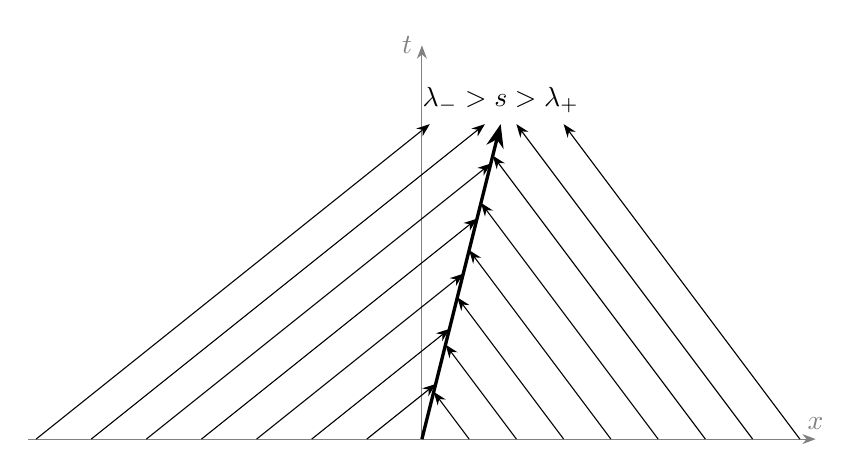
\begin{tikzpicture}[>=Stealth]
	\coordinate (O) at (0, 0);
	\draw[gray] (-5, 0) -- (O);
	\draw[gray,->] (O) -- (5, 0) node[above]{$x$}; % x-axis
	\draw[gray,->] (O) -- (0, 5) node[left ]{$t$}; % t-axis
	% the shock wave
	\draw[->, very thick] (O) -- (1, 4) node[above]{$\lambda_{-}>s>\lambda_{+}$};
	% constant region (left)
	\foreach \y in {0.7, 1.4, ..., 3.5}  \draw[->] (-\y, 0) -- (\y/4, \y);
	\foreach \y in {4.2, 4.9}   \draw[->] (-\y, 0) -- (-\y+5, 4);
	% constant region (right)
	\foreach \y in {0.6, 1.2, ..., 3.6}   \draw[->] (+\y, 0) -- (\y/4, \y);
	\foreach \y in {4.2, 4.8}   \draw[->] (+\y, 0) -- (+\y-3, 4); 
\end{tikzpicture}
\end{document}
